% Torus
\begin{tikzpicture}
  [vertex/.style={circle,fill=black, minimum size=1mm, inner sep=0pt}]
  \draw [>-   ] (-2, 2) -- (-1, 2) (-1, 2) -- ( 0, 2);
  \draw [>-   ] (-2,-2) -- (-1,-2) (-1,-2) -- ( 0,-2);
  \draw [>>-  ] ( 0, 2) -- ( 1, 2) ( 1, 2) -- ( 2, 2);
  \draw [>>-  ] ( 0,-2) -- ( 1,-2) ( 1,-2) -- ( 2,-2);
  \draw [>={Stealth},>- ] ( 2,-2) -- ( 2,-1) ( 2,-1) -- ( 2, 0);
  \draw [>={Stealth},>- ] (-2,-2) -- (-2,-1) (-2,-1) -- (-2, 0);
  \draw [>={Stealth},>>-] ( 2, 0) -- ( 2, 1) ( 2, 1) -- ( 2, 2);
  \draw [>={Stealth},>>-] (-2, 0) -- (-2, 1) (-2, 1) -- (-2, 2);
  \draw [dashed] ( 0, 2) -- ( 0,-2);
  \draw [dashed] ( 2, 0) -- (-2, 0);
  \node at ( 0, 0) [vertex,draw,label= 45:\(x\)] {};
  \node at ( 2, 0) [vertex,draw,label=135:\(z_1\)] {};
  \node at (-2, 0) [vertex,draw,label= 45:\(z_1\)] {};
  \node at ( 0, 2) [vertex,draw,label=315:\(z_2\)] {};
  \node at ( 0,-2) [vertex,draw,label= 45:\(z_2\)] {};
  \node at ( 2, 2) [vertex,draw,label=225:\(y\)] {};
  \node at (-2,-2) [vertex,draw,label= 45:\(y\)] {};
  \node at (-2, 2) [vertex,draw,label=315:\(y\)] {};
  \node at ( 2,-2) [vertex,draw,label=135:\(y\)] {};
\end{tikzpicture}
% \hfill{}
\hspace{2cm}
% link of torus
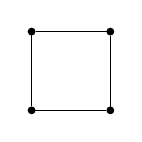
\begin{tikzpicture}
  [
  vertex/.style={
    circle,
    fill=black,
    minimum size=1mm,
    inner sep=0pt
  }
  ]
  \node at (0,0) [vertex] {}
  edge (0,1)
  node at (0,1) [vertex] {}
  edge (1,1)
  node at (1,1) [vertex]{}
  edge (1,0)
  node at (1,0) [vertex]{}
  edge (0,0);
\end{tikzpicture}



%%% Local Variables:
%%% mode: latex
%%% TeX-master: "../Master"
%%% End:
